% !TeX root = ../main.tex

\chapter{Ecuaciones diferenciales difusas}
\begin{chapquote}{Sofia Kovalévskaya}
	``Es imposible ser matemático sin ser un poeta del alma``
\end{chapquote}
En este capítulo se van a explorar los diferentes puntos de vista a los \textbf{conceptos clásicos del cálculo mediante una perspectiva difusa}. Se va a recordar la definición de integral de Riemann, Aumann \& Henstock, y haremos una revisión de la definición de derivada de Hukuhara (\hyperref[def:hukukara]{Diferencia de Hukuhara}). Además, se tratará de la \textbf{versión difusa del teorema fundamental del cálculo} que nos ayudará a tener una mejor visión de la teoría estudiada.

\section{Cálculo difuso para funciones definidas en conjuntos difusos}
Esta sección está basada en el contenido de \cite{fuzzyintro}.
\subsection{Distintas definiciones de derivada}
En primer lugar, vamos a definir los distintos conceptos de derivada difusa.

\subsubsection{La derivada de Hukuhara}
La derivada de Hukuhara está basada en el concepto de \textbf{diferenciabilidad de Hukuhara} para funciones evaluadas en intervalos (\cite{derivatehukuhara})

\begin{definicion}[Diferenciable según Hukuhara]
  Sea $F$ una función definida en un conjunto difuso. Se supone que que los límites:
  
  \[
  \begin{array}{c||c}
    \lim\limits_{h \rightarrow 0^+} \frac{F(x_0 + h) \circleddash_H F(x_0)}{h} & \lim\limits_{h \rightarrow 0^+} \frac{F(x_0) \circleddash_H F(x_0 - h)}{h}
  \end{array}.
  \]
  
  Existen, y son iguales a cierto elemento $F'_H(x_0) \in \mathcal{F}_\mathcal{H}(\IR^n)$, entonces $F$ \textbf{es diferenciable según Hukuhara (H-Diferenciable)} en $x_0$ y se dice que $F'_H(x_0)$ es su derivada en $x_0$ 
\end{definicion}

\begin{ejemplo}[Función constante]
  Sea $F(x)=A$ con $A=(-1;0;1)$, se va a calcular su H-Derivada en un punto arbitrario $x_0 \in \IR$: 
  \[
  F(x_0 + h) \circleddash_H F(x_0) = A \circleddash_H A = 0.
  \]
  \[
  F(x_0) \circleddash_H F(x_0 - h) = A \circleddash_H A = 0.
  \]
  Por tanto, $F_H'(x_0) = 0$
\end{ejemplo}

\begin{ejemplo}[Función lineal]
  \label{ejemplo:hukuhara}
  Sea $F(x)=A x$ con $A=(-1; 0; 1)$, se supone en primer lugar que $x \geq 0$:
  \[
  F(x + h) \circleddash_H F(x) = A(x + h) \circleddash_H A = (-x - h; 0; x+h) \circleddash_H (-x; 0; x) = (-h; 0; h).
  \]
  Análogamente, 
  \[
  F(x) \circleddash_H F(x - h) = (-h; 0; h),
  \]
  de donde,
  \[
  \begin{array}{c||c}
    \lim\limits_{h \rightarrow 0^+} \frac{(-h; 0; h)}{h}=A & \lim\limits_{h \rightarrow 0^+} \frac{(-h; 0; h)}{h}=A
  \end{array}.
  \]
  Por tanto, $F_H'(x) = A $, si $x > 0$. \\
  Por otro lado, si $x<0$, se puede ver que $F(x+h) \circleddash_H F(x)$ no está definido, pues:
  
  \begin{itemize}
  \item $(-x-h; 0; x+h)$ no sería un número triangular, pues $-x-h > x+h$
  \end{itemize}

  Esto se puede ver más fácilmente en un resultado que se muestra a continuación.
\end{ejemplo}

\begin{proposicion}[Construcción de funciones H-Diferenciables \cite{spingerfuzzy}]
  Sea $G$ una función definida en conjuntos difusos tal que $G(x)=B g(x)$ donde $g(x)>0, g'(x)>0$ y $B$ es un número difuso entonces, $G(x)$ es H-Diferenciable, más aún, 
  \[
  G'_H(x) = B g'(x).
  \]
\end{proposicion}

\begin{teorema}[Continuidad de funciones H-Diferenciables \cite{seikkala}] Sea  $F: [a, b] \rightarrow \mathcal{F}_\mathcal{H}(\IR^n)$ una función H-Diferenciable, entonces $F$ es continua en el sentido visto en el Tema 1.
\end{teorema}

\begin{teorema}[Álgebra en derivadas \cite{seikkala}]
  Sean $F, G : [a, b] \rightarrow \mathcal{F}_\mathcal{H}(\IR^n)$ funciones diferenciables y sea $\lambda \in \IR$. Entonces, $(F+G)_H' = F'_H + G_H'$ y $(\lambda F)_H' = \lambda F'_H$.
\end{teorema}

\textbf{Una función H-Diferenciable tiene $\alpha$-corte diferenciables}, sin embargo, \textbf{que todos los $\alpha$-corte sean diferenciables, no implica que la función sea $H$-diferenciable.}

\subsubsection{La derivada de Seikkala}
Ahora se introduce el concepto de derivada de Seikkala, que se usará después para \textbf{introducir un concepto de derivada más fuerte.}

\begin{definicion}[Derivada de Seikkala]
  Sea $F: [a, b] \rightarrow \mathcal{F}_H(\IR)$ si:
  \[
    [(f^-_\alpha)'(x_0), (f^+_\alpha)'(x_0)].
    \]
    existe para cada $\alpha \in [0, 1]$ y define $\alpha$-cortes de un número difuso $F'_S(x_0)$ entonces se dice que $F$ es Seikkala diferenciable en $x_0$ y definimos $F'_S(x_0)$ como la derivada de $F$ en $x_0$.
\end{definicion}

A continuación, se introduce una condición necesaria que servirá de herramienta para relacionar el concepto anteriormente visto de derivada y la derivada de Seikkala.

\begin{teorema}[Condición necesaria Seikkala \cite{seikkala}]
  Si $F: [a, b] \rightarrow \mathcal{F}_\mathcal{H}(\IR^n)$ es H-Diferenciable entonces $f_\alpha^-(x)$ y $f_\alpha^+$ son diferenciables y:
  \[
    [F'(x_0)]_\alpha = [(f_\alpha^-)(x_0), (f_\alpha^+)(x_0)].
    \]
    Entonces, $F$ es diferenciable según Seikkala y la derivada de Seikkala y de Hukuhara coinciden.
\end{teorema}

\subsubsection{La derivada fuertemente generalizada}
El concepto de derivada fuertemente generalizada \textbf{viene a generalizar más aún los conceptos de derivadas ya introducidos por Hukuhara y Seikkala.} \\

Uno de los problemas que nos encontramos con las derivada de Seikkala y Hukuhara es cuando pasa $(f^-_\alpha)'(x_0) \leq (f^+_\alpha)'(x_0)$ (Se puede ver en el Ejemplo \ref{ejemplo:hukuhara}). Si F es Seikkara diferenciable (en particular, si es Hukuhara diferenciable), entonces $(f_{\alpha}^-)'(x) \le (f_{\alpha}^+)'(x)$ y por tanto la diferencia $(f_{\alpha}^+)'(x) - (f_{\alpha}^-)'(x) \ge 0$. Es decir, para todo $\alpha$-corte, la función diámetro$  [F(x)]_{\alpha} = f_{\alpha}^+(x) - f_{\alpha}^-(x)$ es no decreciente. Pero esto es un serio inconveniente: significa que no pueden existir funciones Hukuhara diferenciables que presenten un grado de incertidumbre cada vez menor, o bien cuyo grado de incertidumbre oscile (crezca y decrezca). Para evitar estos problemas, se introdujo el concepto de derivada fuertemente generalizada:

\begin{definicion}[Derivada fuertemente generalizada]
  Sea $F: (a, b) \rightarrow \mathcal{F}_\mathcal{H}(\IR^n)$. Si alguno de los siguientes pares de límites:
  
  \begin{enumerate}
  \item 	
    \[
    \begin{array}{c||c}
      \lim\limits_{h \rightarrow 0^+} \frac{F(x_0 + h) \circleddash_H F(x_0)}{h} & \lim\limits_{h \rightarrow 0^+} \frac{F(x_0) \circleddash_H F(x_0 - h)}{h}
    \end{array}.
    \]
  \item 	
    \[
    \begin{array}{c||c}
      \lim\limits_{h \rightarrow 0^+} \frac{F(x_0 + h) \circleddash_H F(x_0)}{-h} & \lim\limits_{h \rightarrow 0^+} \frac{F(x_0) \circleddash_H F(x_0 - h)}{-h}
    \end{array}.
    \]
  \item 	
    \[
    \begin{array}{c||c}
      \lim\limits_{h \rightarrow 0^+} \frac{F(x_0 + h) \circleddash_H F(x_0)}{h} & \lim\limits_{h \rightarrow 0^+} \frac{F(x_0) \circleddash_H F(x_0 - h)}{-h}
    \end{array}.
    \]
  \item 	
    \[
    \begin{array}{c||c}
      \lim\limits_{h \rightarrow 0^+} \frac{F(x_0 + h) \circleddash_H F(x_0)}{-h} & \lim\limits_{h \rightarrow 0^+} \frac{F(x_0) \circleddash_H F(x_0 - h)}{h}
    \end{array}.
    \]
  \end{enumerate}
  Existen y son iguales a algún elemento $F'_G(x_0)$ de $\mathcal{F}_\mathcal{H}(\IR^n)$, entonces $F$ es diferenciable fuertemente generalizado (o GH) en $x_0$, y $F'_G(x_0)$ es el valor de la derivada. Se denota como GH-Diferenciable.
\end{definicion}
De la definición \textbf{es trivial demostrar que si H-Diferenciable entonces es diferenciable fuertemente generalizado}.

\begin{observacion}
  De la definición anterior se pueden extraer las siguientes conclusiones, basadas en la naturaleza del diámetro de las funciones difusas:
  \begin{enumerate}
  \item Concepto de derivada para funciones con diámetro no decreciente.
  \item Concepto de derivada para funciones con diámetro no creciente.
  \item Concepto de derivada para funciones con diámetro con monotonía arbitraria.
  \item Concepto de derivada para funciones con diámetro con monotonía arbitraria.
  \end{enumerate}
\end{observacion} 

\subsubsection{Otras definiciones}

Para cerrar esta sección, veremos dos conceptos más derivada:

\begin{definicion}[Diferencial de Hukuhara generalizada]
  Sea $F: (a, b) \longrightarrow \mathcal{F}_\mathcal{C}(\IR)$. Si el límite:
  \[
  	\lim\limits_{h \rightarrow 0} \frac{F(x_0 + h) \circleddash_{gH} F(x_0)}{h},
  \]
  existe y pertenece a $\mathcal{F}_\mathcal{C} (\IR)$, entonces $F$ es diferenciable de forma generalizada según Hukuhara (gH diferenciable) en $x_0$, además a $F'_{gH}(x_0)$ se le llama el valor de la derivada de forma generalizada según Hukukahara
\end{definicion}

\begin{definicion}[Diferencial generalizada]
  \label{def:diferencial_generalizada}
  Sea $F: (a, b) \longrightarrow \mathcal{F}_\mathcal{C}(\IR)$. Si el límite:
\[
\lim\limits_{h \rightarrow 0} \frac{F(x_0 + h) \circleddash_{g} F(x_0)}{h},
\]
existe y pertenece a $\mathcal{F}_\mathcal{C} (\IR)$, entonces $F$ es diferenciable de forma generalizada (g diferenciable) en $x_0$, además a $F'_{g}(x_0)$ se le llama el valor de la derivada de forma generalizada
\end{definicion}

Para las definiciones anteriores se puede demostrar la siguiente jerarquía de implicaciones:
\begin{table}[h]
  \centering
  \begin{tabular}{lllllll}
    H-Diferenciable & $\Rightarrow$ & GH-Diferenciable & $\Rightarrow$ & gH-Diferenciable & $\Rightarrow$ & g-Diferenciable
  \end{tabular}
\end{table}

La demostración de lo anterior, como el resto de afirmaciones del capítulo pueden encontrarse en \cite{fuzzyintro}

\subsection{Integral}
La primera propuesta de integral difusa se \textbf{basa en el concepto integral de Aumann \cite{aumannintegral}} para funciones multievaluadas. La definición original podemos verla en \cite{integral1} y \cite{integral2}. \\
Por simplificar, vamos a denotar:
\[
S(G) = \{g : I \rightarrow \IR^n : \text{g integrable}, g(t) \in G(t), \forall t \in I \}.
\]
Vamos a denotar, para cada $G : I \rightarrow \mathcal{P}(\IR^n)$

\subsubsection{Integral de Aumann}
\begin{definicion}[Integral de Aumann]
  La integral de Aumann de una función sobre un conjunto difuso $F : [a, b] \rightarrow \mathcal{F}_C(\IR^n)$ sobre $[a, b]$ se define como: 
  \[
  \left[
    (A) \int_{a}^{b} F(x) dx
    \right]_\alpha = \left\{
  \int_{a}^{b} g(x) dx : g \in S([F(x)]_\alpha)
  \right\}.
  \]
  Para todo $\alpha \in [0, 1]$. La función $F$ se dirá que es integrable sobre $[a, b]$ si $(A) \int_{a}^{b} F(x) dx \in \mathcal{F}_\mathcal{H}(\IR^n)$
\end{definicion}

\subsubsection{Integral de Riemann}
Se puede usar también el concepto clásico de integral para definir una \textbf{integral de Riemann en el ámbito difuso.}

\begin{definicion}[Integral de Riemann]
  La integral de Riemman de una función difusa $F : [a, b] \rightarrow \mathcal{F}_\mathcal{C} (\IR)$ sobre $[a, b]$ es el número difuso $A$ tal que para todo $\varepsilon > 0$ existe un $\delta > 0$ tal que para cualquier partición $\mathcal{P}: = a=x_0 < x_1 < ... < x_n = b$ con $x_i - x_{i-1} < \delta, i = 1, ..., n$ y $\xi_i \in [x_i - x_{i-1}]$
  \[
  	d_\infty \left(
  		\sum_{i=1}^{n-1} F(\xi_i)(x_i - x_{i-1}, A
  	\right) < \varepsilon.
  \]
  La función $F$ se dice que es integrable según Riemann sobre $[a, b]$ y se denota:
  \[
  	(R) \int_{a}^{b} F(x) dx = A.
  \]
\end{definicion}

\subsubsection{Algunos resultados importantes}
En esta sección mostraremos una serie de teoremas de utilidad encontrados en \cite{integral2} que reproducen en cierta manera \textbf{algunas propiedades ya conocidas del cálculo infinitesimal clásico}:

\begin{teorema}
  Si una función $F :  [a, b] \rightarrow \mathcal{F}_\mathcal{H}(\IR)$ es continua según (Definición \ref{def:funcioncontinua}) entonces es integrable. Más aún,
  \[
  \left[
    \int F
    \right]_\alpha = \left[
    \int f_\alpha^-, \int f_\alpha^+
    \right],
  \] para todo $\alpha \in [0, 1]$
\end{teorema}

\begin{teorema}[Cambio de intervalos]
  Sea $F :  [a, b] \rightarrow \mathcal{F}_\mathcal{H}(\IR)$ una función integrable, y supongamos $a \leq x_1 \leq x_2 \leq x_3 \leq b$, entonces:
  \[
  \int_{x_1}^{x_3} F = \int_{x_1}^{x_2} F + \int_{x_2}^{x_3} F.
  \]
\end{teorema}

\begin{teorema}
  Sean $F, G :  [a, b] \rightarrow \mathcal{F}_\mathcal{H}(\IR)$ funciones integrables, entonces:
  
  \begin{enumerate}
  \item $\int F + G = \int F + \int G$.
  \item $\int \lambda F = \lambda \int F$ para cualquier $\lambda \in \IR$.
  \item $d_\infty(F, G)$ es integrable.
  \item $d_\infty(\int F, \int G) \leq \int d_\infty(F, G)$.
  \end{enumerate}
\end{teorema}

\subsection{Teorema fundamental del cálculo}
En la teoría clásica del análisis, \textbf{el teorema fundamental del cálculo nos ofrece una visión bastante fuerte que relaciona las derivadas y las integrales}. En el cálculo difuso tenemos lo mismo, y los siguientes teoremas que vamos a introducir nos \textbf{generalizarán estos teoremas clásicos para casos difusos.}

\begin{teorema}[Teorema fundamental del cálculo difuso\cite{integral2}]
  Sea $F : [a, b] \rightarrow \mathcal{F}_\mathcal{H} (\IR^n)$ una función continua, entonces $G(x) = \int_{a}^{x} F(s) ds$ es H-Diferenciable y además,
  \[
  G'_H(x) = F(x).
  \]
\end{teorema}

\begin{teorema}[\cite{integral2}]
  Sea $F : [a, b] \rightarrow  \mathcal{F}_\mathcal{H} (\IR^n)$ una función H-Diferenciable y sea $F_H'$ su derivada. Supongamos que $F_H'$ es integrable sobre $[a, b]$. Entonces,
  \[
  F(x) = F(a) + \int_{a}^{x}F_H'(s) ds,
  \]
  para todo $x \in [a, b]$.
\end{teorema}

También se puede enunciar un teorema un teorema parecido al anterior, pero esta vez exigiendo que la función es diferenciable fuertemente generalizada (2):

\begin{teorema}[\cite{fundamental}]
  Sea $F : [a, b] \rightarrow  \mathcal{F}_\mathcal{H} (\IR^n)$ una función diferenciable fuertemente generalizada (2) y sea $F_H'$ su derivada. Supongamos que esta es integrable sobre $[a, b]$. Entonces,
  \[
  F(x) = F(a) + \int_{a}^{x}F_H'(s) ds,
  \]
  para todo $x \in [a, b]$.
\end{teorema}

\section{Ecuaciones diferenciales difusas}
Del mismo modo que \textbf{hay varios acercamientos al concepto de derivada}, no podía ser menos el concepto de ecuación diferencial difusa. En esta sección \textbf{vamos a tratar los distintas formas de acercarse a los conceptos de ecuación diferencial difusa}. Esta sección toma como referencia \cite{fuzzyapproaches}

\subsection{Introducción}
En esta sección vamos a empezar planteando un problema de valor inicial difuso de la misma manera que se introducen las ecuaciones diferenciales clásicas. Dado un número difuso $X_0$, se trata de hallar una función $X:[0,T] \rightarrow F_H(U)$ tal que:

\begin{equation}
  \label{def:edf}
  X'(t) = f(t, X(t)), ~ X(0) = X_0,
\end{equation}
donde $f : [O, T] \times \mathcal{F}_\mathcal{H}(\IU) \rightarrow \mathcal{F}(\IR^n)$ se obtiene mediante el \hyperref[def:zadeh]{principio de extensión de Zadeh} aplicada a una función continua $g : [0, T] \times U \rightarrow \IR^n$. Además, $f$  es continua por ser $g$ continua, aplicando \hyperref[teorema:contfuzzy]{Teorema \ref*{teorema:contfuzzy}} se puede concluir:
\[
	[f(t, X)]_\alpha = g(t, [X]_\alpha).
\]
Se puede \textbf{asociar a esta ecuación diferencial difusa una ecuación diferencial ordinaria:}
\begin{equation}
	\label{eq:edo}
	x'(t) = g(t, x(t)), ~ x(0) = c.
\end{equation}

Así, decimos que $X(t)$ es una solución difusa de (3.1) en (el sentido del principio de extensión) si existe una solución $x(t,c)$ de (3.2) y, para cada t fijo, se tiene que

\[
X(t) = \hat x (t, X_0),
\]
donde $\hat x(t, X_0)$ es el resultado de aplicar el principio de extensión de Zadeh respecto al parámetro c a la función x(t,c).
\subsection{Teorema de equivalencia entre EDO y EDD}

A continuación, se ofrece un teorema que dará una relación entre ecuaciones diferenciales difusas y ordinarias.

\begin{teorema}[Equivalencia entre EDO y EDD \cite{fuzzyapproaches1}]
	\label{teorema:equivalencia}
	Sea $U$ un conjunto abierto sobre $\IR^n$ y supongamos que $[X_0]_\alpha \subset U$ con $\alpha \in [0, 1]$. Sea $g$ una función continua, y suponga que para cada $c \in U$ existe una única solución $x(\cdot, c)$ del problema (\ref{eq:edo}) y también que $x(t, \cdot)$ es continúa para todo $t \in [0, T]$ fijado. Entonces, existe una única solución difusa $X(t) = \hat{x}(t, x_0)$ del problema (\ref{def:edf})
\end{teorema}
El resultado anterior es muy potente, \textbf{permitirá utilizar métodos numéricos ya conocidos para resolver ecuaciones diferenciales difusas fácilmente.}

Para ver la potencia del Teorema anterior, se introducirán una serie de ejemplos:

\begin{ejemplo}
	Se plantea la siguiente ecuación diferencial difusa con valores iniciales:
	\[
		\left\{
			\begin{array}{ccc}
				X' & = & - X(t) \\
				X(0) & =  & C
			\end{array}
		\right.,
	\]
	
	donde $C$ representa un número difuso arbitrario. A continuación se construye el problema ordinario asociado al problema difuso de la misma manera que se hace al inicio de esta sección;
	
	\[
		\left\{
			\begin{array}{ccc}
				x' & = & - x(t) \\
				x(0) & =  & c
			\end{array}
		\right..
	\]
	
	Es bien conocido que este problema de valores iniciales tiene la siguiente solución:
	\[
		x(t, c) = c e^{-t}.
	\]
	
	Por tanto, dado que $x(t, c)$ es continúa para cada $t, c \in \IR$ se puede aplicar el \hyperref[teorema:equivalencia]{Teorema de equivalencia} y tenemos que la solución del problema difuso es:
	\[
		X(t) = C \cdot e^{-t}.
	\]
\end{ejemplo}

\begin{ejemplo}
	Se plantea ahora un problema un tanto más interesante:
	\[
		\left\{
			\begin{array}{ccc}
				X' & = & X^2(t) \\
				X & =  & C
			\end{array}
		\right.,
	\]
	
	donde esta vez $C$ es un número difuso triangular:
	\[
		C(y) = \left\{
			\begin{array}{ccc}
				3 - y & si & 2 \leq y \leq 3 \\
				y - 1 & si & 1 \leq y \leq 2 \\
				0 
			\end{array}
		\right. .
	\]
	El problema ordinario (o determinístico asociado) viene dado por:
	\[
		x'(t) = x^2(t), ~ x(0) = c
	\]
	y la solución de este problema viene dado por:
	\[
		x(t, c) = \frac{c}{1-tc},
	\]
	para cada $t \in [0, \frac{1}{3})$ fijado, la función $(x, t)$ es continua respecto a $c$, entonces se puede aplicar el \hyperref[teorema:equivalencia]{Teorema de equivalencia} y podemos concluir que existe una única solución difusa dada por $X(t) = \hat{x}(t, X_0)$. Se observa que es posible calcular la solución difusa aplicando directamente el principio de extensión de Zadeh y el \hyperref[teorema:contfuzzy]{Teorema \ref*{teorema:contfuzzy}}. Por tanto, se pueden calcular los $\alpha$-cortes de la siguiente forma para cada $\alpha \in [0, 1]$:
	
	\[
		\begin{array}{ccc}
			[X(t)]_\alpha & = & [\hat{x}(t, X_0)]_\alpha \\
			& = & x(t, [X_0]_\alpha) \\
			& = & x(t, [1+\alpha, 3-\alpha]) \\
			& = & [x(t, 1+\alpha), x(t, 3-\alpha)] \\
			& = & \left[
				\frac{1+\alpha}{1-t-t\alpha}, \frac{3-\alpha}{1-3t + t\alpha}
			\right]
		\end{array}.
	\]
	
    \begin{figure}[h]
	\centering
		\frame{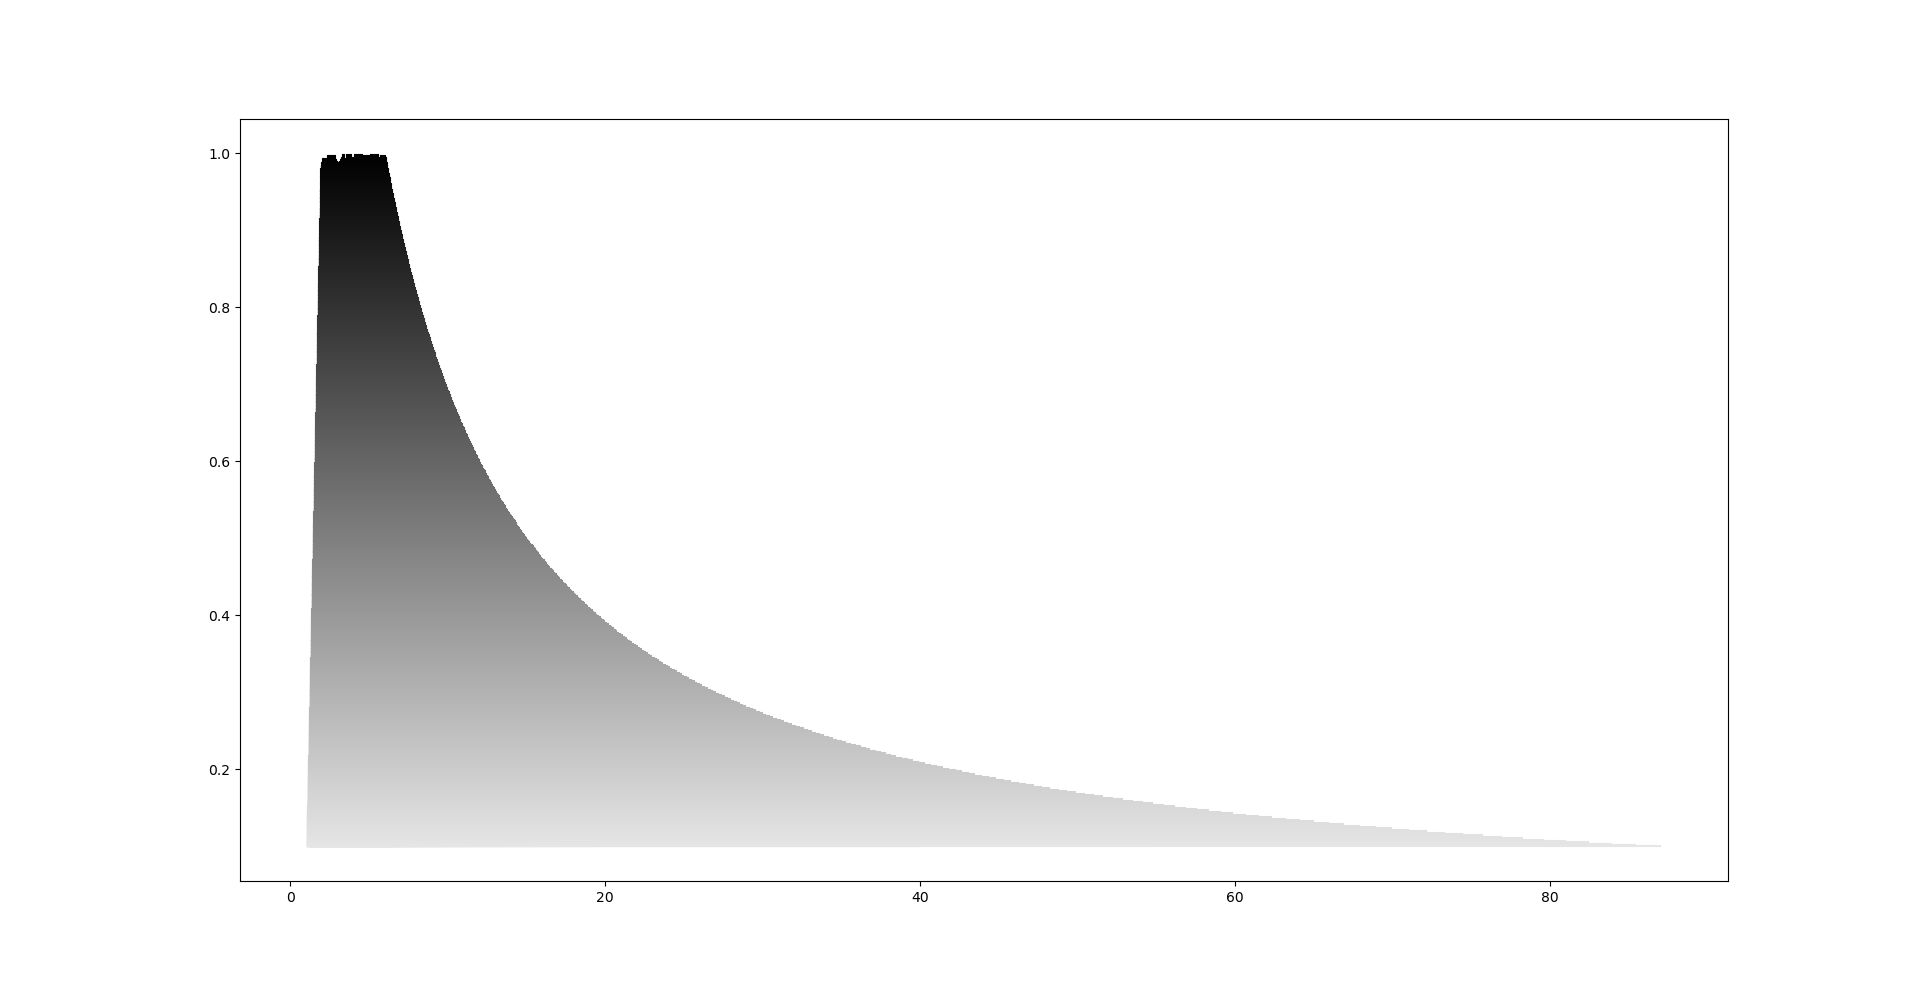
\includegraphics[width=\textwidth]{zadeh_edf}}
		\caption{Gráfica de función de pertenencia}
		\label{fig:solucion_difusa}
	\end{figure}
\end{ejemplo}

\subsection{Inclusiones diferenciales}
Esta sección está basada en la teoría que se puede encontrar en \cite{fuzzyintro}, que a su vez se fundamenta en los artículos  \cite{inclusionesdif1}, \cite{inclusionesdif2} y \cite{inclusionesdif3}.\\
En estos artículos Hüllermeier y Diamond interpretan las  \hyperref[def:edf]{Ecuaciones Diferenciales Difusas} como una familia inclusiones diferenciales:

\begin{equation}
	\label{def:familiainclusionesdif}
	y'_\alpha(t) = g(t, y_\alpha(t)), ~ y_\alpha(0) \in [X_0]_\alpha, ~ 0 \leq \alpha \leq 1.
\end{equation}

Bajo unas determinadas hipótesis, podemos afirmar:
\[
	\mathcal{A}_\alpha = \{y_\alpha | y_\alpha ~ \text{es una solución de la \hyperref[def:familiainclusionesdif]{Familia de inclusiones diferenciales}}\},
\]
son los $\alpha$-cortes de un determinado conjunto difuso y se le llaman soluciones del problema dado por la \hyperref[def:familiainclusionesdif]{Familia de inclusiones diferenciales}

A continuación se ofrece un teorema análogo al teorema que se vio en la sección introductoria \hyperref[teorema:equivalencia]{Teorema de Equivalencia entre EDO y EDF}
\begin{teorema}[\cite{fuzzyapproaches1}]
	Sea $U$ un conjunto abierto en $\IR^n$ y sea $X_0 \in \mathcal{F}(U)$. Dada la función $g$ continua, para cada $c \in U$ existe una única solución $x(\cdot, c)$ del problema \ref{eq:edo} y que $x(t, \cdot)$ es continúa en $U$ para cada $t \in [0, T]$. Entonces, la solución difusa del problema (\ref{def:edf}) (en el sentido del principio de extensión de Zadeh) y las soluciones del del problema de \hyperref[def:familiainclusionesdif]{Familia de inclusiones diferenciales} coinciden, es decir;
	\[
		X(t) = \mathcal{A}(t),
	\]
	para todo $t \in [0, T]$.
\end{teorema}

\section{Ecuaciones en derivadas parciales}
Hasta aquí toda nuestra discusión se ha enfocado en tratar de desarrollar una teoría para plantear y resolver ecuaciones diferenciales difusas.

En esta sección se va a desarrollar un método para resolver ecuaciones en derivadas parciales con condiciones de contorno difusas.

\subsection{Método de líneas (MOL) \cite{MOL}}
Para desarrollar este método, se va a exponer un ejercicio.

Se considera el siguiente problema, ligado a una ecuación parabólica, con $x \in [0, 1]$ y $t > 0$

\[
	\frac{\delta u(x, t)}{\delta t} = \frac{\delta^2 u (x, t)}{\delta x^2}
\]

Donde debido a las limitaciones de nuestros instrumentos de medidas, no somos capaces de dar unas condiciones de contornos exactas, y consideramos un número difuso $\epsilon$ para representar este error en la medida. Y definimos las condiciones de contornos de la siguiente forma:

\[
u(x, 0) = \epsilon \sin{\pi x}
\]
\[
u(0, t) = u(1, t) = 0
\]

\subsubsection{Desarrollo del método de líneas}
Consideramos la discretización de $[0, 1]$ dada por $\mathcal{P}_N = \displaystyle \left\{\frac{n}{N} :  n\in \mathbb{Z}, 0 \leq n \leq N \right\}$ y  $h=\frac{1}{N}$.

Definimos $(x_n, t)$ con $x_n \in \mathcal{P}_N$ y $t>0$ para algún $N > 0$   como la semirrecta vertical. Consideramos en esta recta una función de $t>0$ como:
\[
	u_n(t) = u(x_n, t)
\]

Observemos que por las condiciones de contorno tenemos:
\[
	u_0(t) = u(0, t) = 0
\]
\[
	u_N(t) =u(1, t) = 0
\]

Observemos  que hemos conseguido una discretización de una variable, pero sigue siendo continua para la variable $t$.  

Consideremos ahora para un $t \in [0, +\infty]$
\[
f: x \longrightarrow u(x, t)
\]

Esta función cumple:
\[
	\frac{\delta u(x, t)}{\delta t} = f''(x)
\]

En particular,
\[
\frac{\delta u(x_n, t)}{\delta t} = f''(x_n)
\]
Aproximamos $\frac{\delta u(x_n, t)}{\delta t}$  mediante:

\[
\frac{\delta u(x_n, t)}{\delta t} = \frac{u(x_{n-1}, t)  -2 u(x_{n}, t )+ u(x_{n+1}, t)}{h^2} + \mathcal{O}(h^2)
\]

Agrupando las soluciones escalares en el vector de funciones:
\[
	u(t) = (u_1(t), u_2(t), ..., u_{N-1} (t))
\]

Teniendo en cuenta que las funciones $u_0(t)$ y $u_N(t)$ son condiciones de contorno, idénticamente nulas, podemos escribir lo siguiente:

\[
	u' = \frac{1}{h^2} A u
\]

Donde A es la matriz:

\[
	A= \left[
		\begin{array}{cccc}
			-2 & 1 & 0 & \cdots \\
			1 & -2 & 1 & \cdots \\
			0 & 1 & -2 & \cdots \\
			\vdots & \vdots & \vdots & \ddots
		\end{array}
	 \right]
\]

Por otra parte, la condición inicial para $u$:
\[
	u(x, 0) = \epsilon \sin{\pi x}
\]
Para $u_n(0)$ podemos escribir:
\[
	u_n(0) = u(x_n, 0) = \epsilon \sin{\pi \ n h}
\]

Con este procedimiento hemos conseguido escribir nuestra ecuación en derivadas parciales como una ecuación diferencial ordinaria.

La resolución numérica de este problema se puede llevar a cabo mediante métodos clásicos como Runge-Kutta.